% Shared Beamer style and diagrams. Compile language files with XeLaTeX.
\documentclass[aspectratio=169,10pt]{beamer}
\usepackage[no-math]{fontspec}
\setsansfont{Malgun Gothic}
\setmainfont{Malgun Gothic}
\setmonofont{Consolas}
\XeTeXlinebreaklocale "ko"
\XeTeXlinebreakskip=0pt plus 0.5pt
\usepackage{amsmath,graphicx,booktabs,tikz}
\usefonttheme{professionalfonts}
\usefonttheme[onlymath]{serif}
\usetikzlibrary{arrows.meta,positioning,calc,shapes.geometric}
\definecolor{ink}{HTML}{142938}
\definecolor{accent}{HTML}{155F85}
\definecolor{pale}{HTML}{E7F0F7}
\definecolor{collision}{HTML}{A03336}
\setbeamercolor{normal text}{fg=ink,bg=white}
\setbeamercolor{frametitle}{fg=ink}
\setbeamercolor{structure}{fg=accent}
\setbeamerfont{frametitle}{size=\Large,series=\bfseries}
\setbeamertemplate{navigation symbols}{}
\setbeamertemplate{footline}{\hfill{\color{accent}\scriptsize RMFS Architecture\quad \insertframenumber\ /\ \inserttotalframenumber}\hspace{5mm}\vspace{3mm}}
\setbeamersize{text margin left=7mm,text margin right=7mm}
\hypersetup{pdftitle={RMFS Architecture}}
\tikzset{
 phase/.style={ellipse,draw=accent,fill=pale,minimum width=23mm,minimum height=10mm,align=center,font=\small},
 terminal/.style={phase,draw=collision,fill=red!5},
 flow/.style={-{Stealth[length=2mm]},draw=accent,thick},
 ext/.style={flow,dashed},
 crash/.style={ext,draw=collision},
 lab/.style={font=\scriptsize,align=center,fill=white,inner sep=1.5pt},
 module/.style={draw=accent,fill=pale,rounded corners=2pt,minimum width=34mm,minimum height=13mm,align=center}
}
\newcommand{\MRobotDiagram}{%
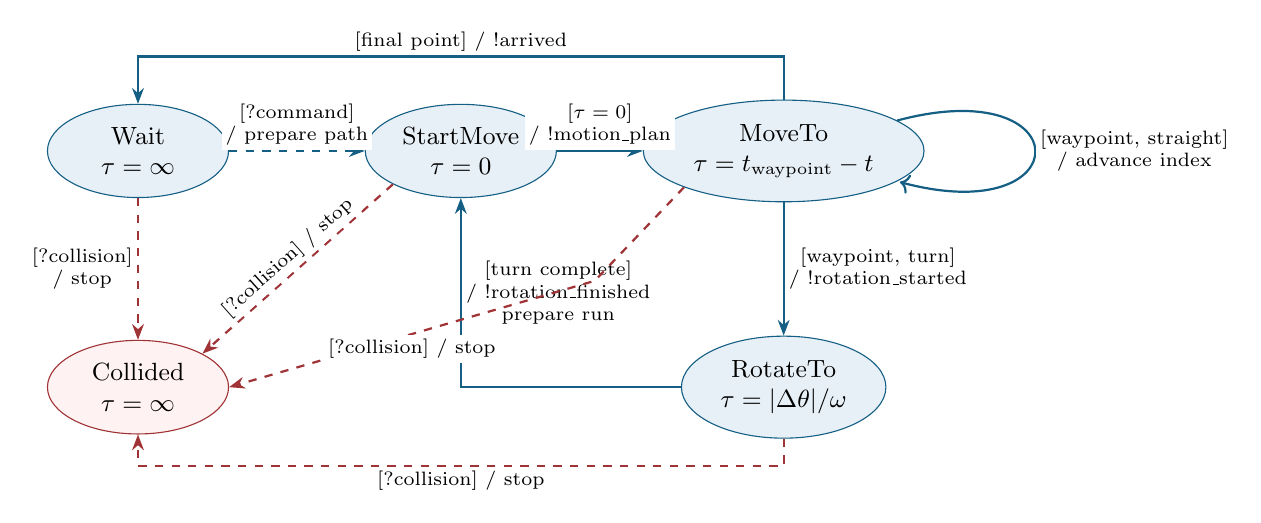
\begin{tikzpicture}[x=1cm,y=1cm]
\node[phase] (w) at (0,3) {Wait\\$\tau=\infty$};
\node[phase] (s) at (4.1,3) {StartMove\\$\tau=0$};
\node[phase] (m) at (8.2,3) {MoveTo\\$\tau=t_{\rm waypoint}-t$};
\node[phase] (r) at (8.2,0) {RotateTo\\$\tau=|\Delta\theta|/\omega$};
\node[terminal] (c) at (0,0) {Collided\\$\tau=\infty$};
\draw[ext] (w)--node[lab,above]{[?command]\\ / prepare path}(s);
\draw[flow] (s)--node[lab,above]{[$\tau=0$]\\ / !motion\_plan}(m);
\draw[flow] (m) edge[loop right] node[lab,right]{[waypoint, straight]\\ / advance index}(m);
\draw[flow] (m)--node[lab,right]{[waypoint, turn]\\ / !rotation\_started}(r);
\draw[flow] (r.west)--(4.1,0) -- node[lab,right]{[turn complete]\\ / !rotation\_finished\\prepare run}(s.south);
\draw[flow] (m.north)--(8.2,4.2)--node[lab,above]{[final point] / !arrived}(0,4.2)--(w.north);
\draw[crash] (w.south)--node[lab,left]{[?collision]\\ / stop}(c.north);
\draw[crash] (s.south west)--node[lab,above,sloped]{[?collision] / stop}(c.north east);
\draw[crash] (m.south west)--(5.8,1.35)--node[lab,below]{[?collision] / stop}(c.east);
\draw[crash] (r.south)--(8.2,-1)--node[lab,below]{[?collision] / stop}(0,-1)--(c.south);
\end{tikzpicture}}
\newcommand{\PSensorDiagram}{%
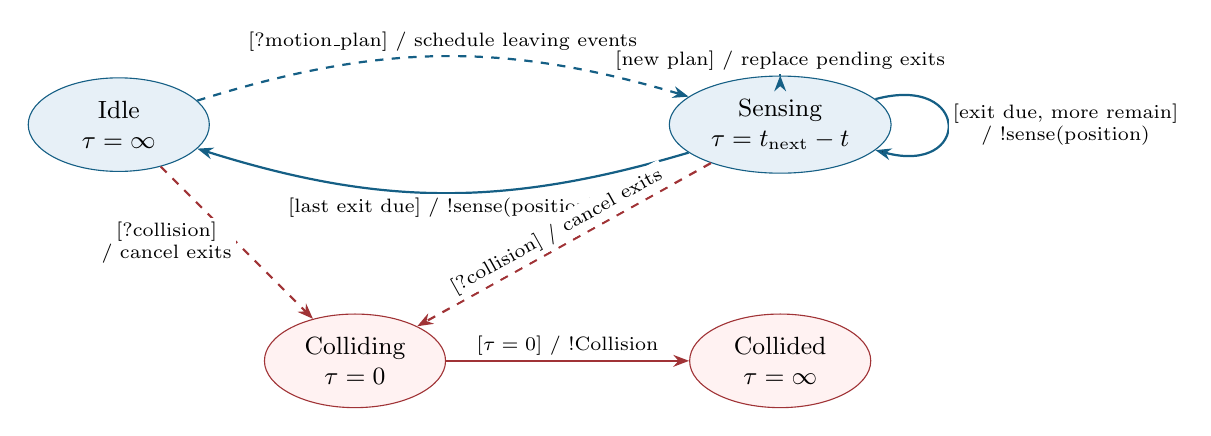
\begin{tikzpicture}[x=1cm,y=1cm]
\node[phase] (i) at (0,3) {Idle\\$\tau=\infty$};
\node[phase] (s) at (8.4,3) {Sensing\\$\tau=t_{\rm next}-t$};
\node[terminal] (g) at (3,0) {Colliding\\$\tau=0$};
\node[terminal] (c) at (8.4,0) {Collided\\$\tau=\infty$};
\draw[ext] (i) to[bend left=17] node[lab,above]{[?motion\_plan] / schedule leaving events}(s);
\draw[flow] (s) to[bend left=17] node[lab,below]{[last exit due] / !sense(position)}(i);
\draw[flow] (s) edge[loop right,looseness=5] node[lab,right]{[exit due, more remain]\\ / !sense(position)}(s);
\draw[ext] (s.north) to[out=120,in=60,looseness=3] node[lab,above]{[new plan] / replace pending exits}(s.north);
\draw[crash] (i)--node[lab,left]{[?collision]\\ / cancel exits}(g);
\draw[crash] (s)--node[lab,sloped,above]{[?collision] / cancel exits}(g);
\draw[flow,draw=collision] (g)--node[lab,above]{[$\tau=0$] / !Collision}(c);
\end{tikzpicture}}
\newcommand{\Profiles}{%
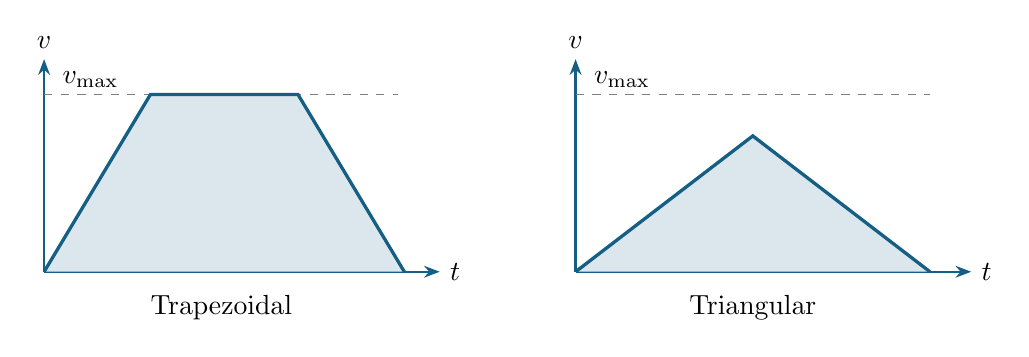
\begin{tikzpicture}[x=0.75cm,y=0.75cm]
\foreach \x in {0,9}{
 \draw[flow] (\x,0)--++(6.7,0) node[right] {$t$};
 \draw[flow] (\x,0)--++(0,3.6) node[above] {$v$};
 \draw[dashed,gray] (\x,3)--++(6,0);
}
\fill[accent!15] (0,0)--(1.8,3)--(4.3,3)--(6.1,0)--cycle;
\draw[accent,very thick] (0,0)--(1.8,3)--(4.3,3)--(6.1,0);
\fill[accent!15] (9,0)--(12,2.3)--(15,0)--cycle;
\draw[accent,very thick] (9,0)--(12,2.3)--(15,0);
\node at (3,-.6) {Trapezoidal};
\node at (12,-.6) {Triangular};
\node[anchor=west] at (.15,3.25) {$v_{\max}$};
\node[anchor=west] at (9.15,3.25) {$v_{\max}$};
\end{tikzpicture}}
\newcommand{\shot}[1]{\includegraphics[width=\linewidth,height=5.65cm,keepaspectratio]{assets/#1.png}}

